%!TEX root = ../../report.tex

\subsubsection{Tiling} % (fold)
\label{ssub:tiling}

A common solution to give realism to 3D objects is the application of textures. One problem is that this textures take a lot of memory space. To work around this problem an easy solution is to have a small texture piece, a tile, and repeat it throughout the objects, this is called tiling. Or as defined in \cite{TilingWOLFRAM}: ``A plane-filling arrangement of plane figures or its generalisation to higher dimensions.".  This means, the result of constructing a plane from a finite set of ``tiles". 

If this technique is used naively, commonly result in not very homogeneous textures. It depends much on the set of tiles that are used. If the borders of all the tiles are all the same the result is always homogeneous. Increase if the borders are very different the chances of getting a non-uniform texture rises. Figure~\ref{fig:TIrregulartexture}, from \cite{ProcWorld} shows how a bad structured tiling system produces a non-homogeneous texture.  


\begin{figure}[htbp]
	\centering
	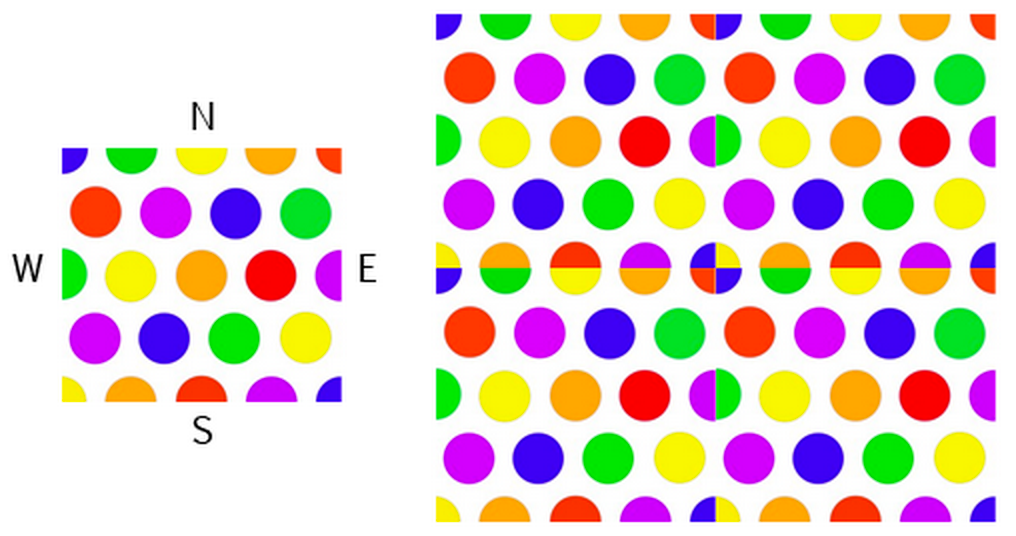
\includegraphics[width=0.95\textwidth]{img/Theory/Tiling/iregular.png}
	\caption{One tile and an irregular pattern}
	\label{fig:TIrregulartexture}
\end{figure}


To make uniform planes, the boundary of each tile must be coherent, i. e., the borders of connecting tiles have to match. Given a single tile, the so-called first corona is the set of all tiles that have a common boundary point with the tile (including the original tile itself). From that, the simplest method to create a homogeneous texture is to connect each tile with one that belongs to its first corona.

The easy, most simple solution is to make sure that all the tiles have the same borders all around. With this property it is guaranteed that any created texture will be homogeneous. But this solution does not provide much irregularity and the results present repeating patterns. 



\emph{Wang Tiles \cite{Cohen2003}} is a solution named after Mr Hao Wang that predicted that tiling was not possible. It received his name, not only for him being wrong, but because the proof that this is possible uses much of the work he did trying to prove the impossibility. This process allows tiling with an arbitrary number of different vertical and horizontal borders and from that calculate the set of tiles that are needed to create a full texture without inconsistencies. 



\begin{figure}
        \centering
		%\begin{subfigure}[b]{0.4\textwidth}
			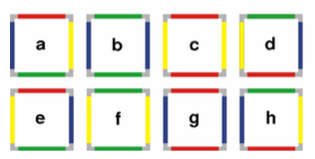
\includegraphics[width=0.45\textwidth]{img/Theory/Tiling/tiles.png}
		%	\caption{a)}
		%	\label{fig:TTileSet}
		%\end{subfigure}
        ~ ~%add desired spacing between images, e. g. ~, \quad, \qquad, \hfill etc.
          %(or a blank line to force the subfigure onto a new line)
		%\begin{subfigure}[b]{0.4\textwidth}
			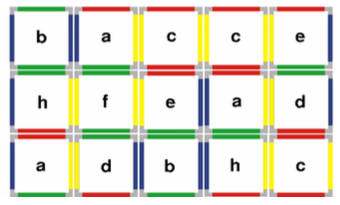
\includegraphics[width=0.45\textwidth]{img/Theory/Tiling/plane.png}
		%	\caption{b)}
		%	\label{fig:TPlanePortion}
		%\end{subfigure}
        \caption{a) Eight Wang Tiles b) Portion of a plane}
        \label{fig:WangTiles}
\end{figure}

So the process is to assign colors to the tiles borders and then matching colored borders are aligned forming a plane.

% paragraph wang_tiles_ (end)

As you might have noticed, the inner content of the tiles are not a problem. As we are trying to create the uniform textures by arranging this smaller pieces only the borders matter, so we can create a set of tiles with the same borders and whatever inner content we want. With this technique the result can be much more irregular and more natural looking textures.


\emph{Corner Tiles \cite{LD06AWTCECC}}. The vanilla wang tiles have problems in the diagonals that are not taken into account. They are the confrontation between four tiles which leads to less homogeneous texture if we the borders do not match. By using the corners, the problem goes to the sides, that despite being larger, are only the confrontation between two tiles and therefore it leads to a more homogeneous texture.
 % paragraph corner_tiles (end) 


% \paragraph{Genetic tile generation} % (fold)
% \label{par:genetic_tile_generation}
% “The bottom line for me is, Wang tiles are amazing things until you try to use them seriously. They work great for stuff you can synthesise from the ground up. If you are trying to mix samples from real life, get ready for some trouble.” \cite{ProcWorld}
%\url{http://procworld.blogspot.pt/2013/01/tile-genetics.html}
% paragraph Genetic tile generation (end)




% subsubsection tiling (end)